 \chapter{Asynchronous programming strategies and their performance}
 \label{chap:async}
\section{Asynchronous programming}
\label{sec:async}
Asynchronous programming is the programming model in which operations that must be executed are interleaved with one another within the single control thread. An analogy to it can be package multiplexing in a Computer Networks. 

In contrast multi-threaded systems are synchronous and allow execution of one task per unit of time blocking execution of other tasks until programmer will perform explicit control delegation to another task.

Generally, asynchronous systems are easier to control and to develop rather then multi-threaded, and  they perform better then synchronous in following cases\cite{asyncArticle}:
 \begin{itemize}
	\item Large number of tasks and, at least, one task likely to make progress;
	\item A lot of I/O operations;
	\item Tasks are independent of one another;
 \end{itemize}



\subsection{node.js}
\label{subsec:node}
node.js is an asynchronous event-driven framework designed to build scalable network applications.
node.js is similar in design to and influenced by systems like Ruby's Event Machine or Python's Twisted with the difference that it presents the event loop as a language construct but not as a library\cite{nodejsabout}.

node.js as a framework has powerful ecosystem - npm which consists of three parts. \textit{npm} - package manager for node.js, \textit{npm Registry} - public collection of packages of open-source code, \textit{npm command line client} which allows developers to install and publish those packages. The diagram (Fig.: \ref{fig:npmStat}) states the comparison of npm with other package, for more up to date information please visit \url{http://www.modulecounts.com/}.
\begin{figure}[ht]
	\label{fig:npmStat}
	\centering
	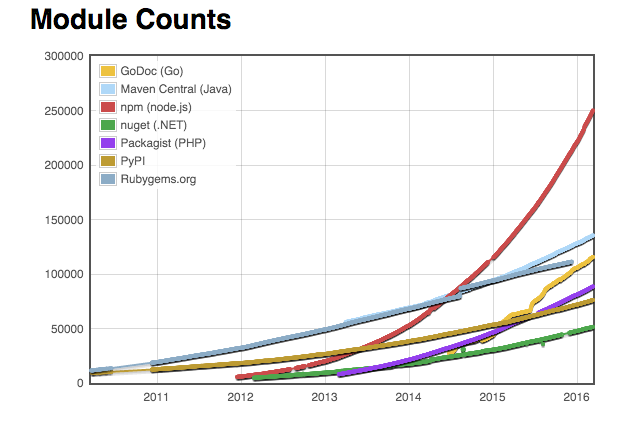
\includegraphics[width=\textwidth]{grafiken/modulecounts.png}
	\caption{npm comparison with other package managers\cite{moduleCounts}}
\end{figure}

At the same time there is a downside of such ecosystem. The case of \textit{left-pad}, the module which was deleted from the npm due to copyright concerns caused by the failure during the build process for thousands of projects\cite{npmDown}. Moreover, there are three factors explained by Sam Saccone \cite{npmHydra} \cite{npmSoft}. All of them make npm a root source of hackers attack since all life-cycle scripts executed by installed packages are executed with same privilege level as a user invoked their installation. The \textit{first} reason is caused by the usage of SemVer for the version controlling which does not lock dependencies to a specific version The\textit{ second }reason is the lack of automatic npm user log-out.  npm can run arbitrary scripts on install it means that any user who is currently logged in and types npm install allows any module to execute arbitrary publish commands. The \textit{third} reason is dependent on the fact that a singular npm registry is used by large majority of the node.js ecosystem on a daily basis.

General suggestions to overcome problems for project developers and maintainers are following:
\begin{itemize}
	\item disable life-cycle scripts during update/install process;
	\item lock down all dependencies versions either manually or using shrinkwrap package \url{https://docs.npmjs.com/cli/shrinkwrap}
	\item store dependencies locally and use them as a part of source code being deployed.
\end{itemize}


node.js applications are written in javascript - a lightweight dynamic scripting multi-paradigm language with first-class functions and prototype-based inheritance which provides both object-oriented and functional programming approaches\cite{mdnJS}.

%When it comes to inheritance, JavaScript has only one construct: objects\cite{mdnProto}.
%This can be called classless, prototype-oriented, or instance-based programming\cite{mdnOOP}. Each object has an internal link to another object called its \textit{prototype}. That prototype object has a prototype of its own, and so on until an object is reached with \textbf{null} as its prototype. \textbf{null}, by definition, has no prototype and acts as the final link in this prototype chain. JavaScript objects are dynamic "bags" of properties (referred to as own properties). When trying to access a property of an object, the property will not only be sought on the object but on the prototype of the object, the prototype of the prototype, and so on until either a property with a matching name is found or the end of the prototype chain is reached\cite{mdnProto} This type of inheritance provide objects inherit both instance and class methods together with properties.

 
The high-level architecture of node.js looks as following:(\ref{fig:nodeArch}). 
\begin{figure}[ht]
  	\label{fig:nodeArch}
    \centering
    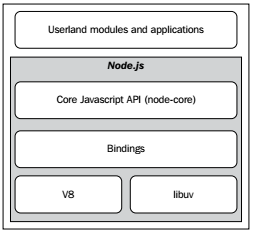
\includegraphics[scale=1.0]{grafiken/nodeArchitecture.png}
     \caption{Node.js architecture \cite{nodejsbook}}
  \end{figure}

\textit{Node core} is a javascript library (called node-core) that implements the high-level node.js API.

\textit{Bindings} responsible for wrapping and exposing \textit{libuv} and other low-level functionality to javascript.\cite{nodejsbook}

\textit{Non blocking I/O} provided by libuv\cite{nodejsabout}\cite{nodejsbook}. 
Which is "a multi-platform support library with a focus on asynchronous I/O. "\cite{libuv} with following properties\cite{libuvBasic}:
\begin{itemize}
\item Abstract operations, not events
\item Support different nonblocking I/O models
\item Focus on extendability and performance
\end{itemize}

\textit{V8/Chakra} the JavaScript engine originally developed by Google for the Chrome browser/ Microsoft for IE 9 browser"\cite{nodejsbook} 



\subsection{Event handling}
\label{subsec:event}
An event is a core concept of asynchronous programming in node.js. All objects that emit events allows one or more functions to be attached to named events emitted by the object. When an event is emitted all the functions attached to that specific event are called synchronously\cite{events}. Node.js  event handler is an implementation of \textit{reactor pattern}. The illustration of process life-cycle is shown in Fig. \ref{fig:nodeEvent}:

\begin{figure}[ht]
  	\label{fig:nodeEvent}
    \centering
    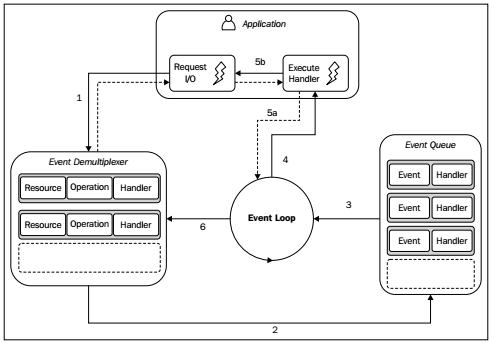
\includegraphics[width=\textwidth]{grafiken/nodeEventHandling.png}
     \caption{Node.js event handling system \cite{nodejsbook}}
  \end{figure}

\begin{enumerate}
	\item The application generates a new I/O operation by submitting a request to the \textit{Event Demultiplexer}. The application also specifies a \textit{listener}, which will be invoked when the operation completes. Submitting a new request to the Event Demultiplexer is a non-blocking call and it immediately returns the control back to the application.
	\item When a set of I/O operations complete, the Event Demultiplexer pushes the new events into the \textit{Event Queue}.
	\item At this point, the \textit{Event Loop} iterates over the items of the Event Queue.
	\item For each event, the associated listener is invoked.
	\item The listener, which is part of the application code, will give back the control to the Event Loop when its execution completes. However, new asynchronous operations might be requested during the execution of the listener, causing new operations to be inserted in the Event Demultiplexer, before the control is given back to the Event Loop.
	\item When all the items in the Event Queue are processed, the loop will block again on the Event Demultiplexer which will then trigger another cycle.
\end{enumerate}

\section{Asynchronous handling strategies}
\label{sec:asyncstrat}
\subsection{Declarative}
The presence of functions as the first class citizens in javascript allows direct usage of functions for handling asynchronous program behavior. \textit{Callbacks} are default handlers for the reactor pattern described before. They are similar to \textit{visitor pattern} in OOP or continuation-passing-style from Functional Programming. They represent an operation to be performed on the elements of an object structure and they let define a new operation without introducing any changes to the definition of the object. 
By convention callbacks must be passed as the last argument and accept two parameters, the first is an error and the second is a data to be processed further.

There are two main negative sides of using callbacks. One of them is so-called \textit{callback hell} occurs due to the abundance of closures and in-place callback definitions. This makes the code hard to be read because of high level nesting, as well as written due to a scope of nesting and difficult to manage because of possible memory leaks created by closures. Another negative side is called \textit{releasing Zalgo}\cite{zalgo}, it occurs only in case of inconsistent function behavior when under some hidden conditions a function performs a synchronous action but some under other - asynchronous.

\subsection{Imperative}
The further explanation is based on the \textit{concept of duality} (Fig. \ref{fig:dualityMatrix}) showed by Erik Meijer \url{https://channel9.msdn.com/Events/Lang-NEXT/Lang-NEXT-2014/Keynote-Duality} and used by Kris Koval in his \textit{General Theory of Reactivity} \url{https://github.com/kriskowal/gtor/}.

\begin{figure}[ht]
	\label{fig:dualityMatrix}
	\centering
	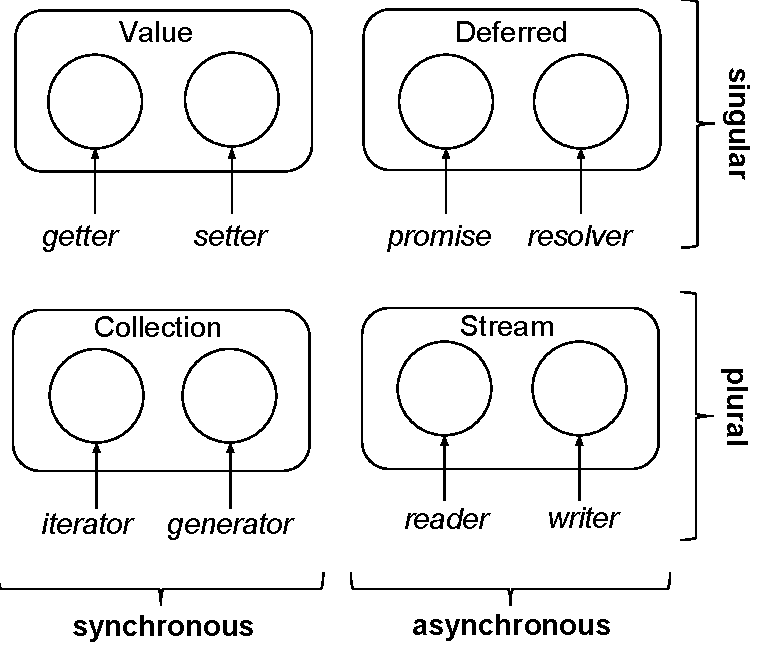
\includegraphics[scale = 0.5]{grafiken/dualityMatrix}
	\caption{Duality Matrix \cite{gtor}}
\end{figure}

The explanation of asynchronous patterns in this chapter will be made as two-dimensional mapping. The first dimension is a time where things can be \textit{synchronous} and \textit{asynchronous}. Another dimension of space where mapping is done between \textit{singular} and \textit{plural}.

Often during communication the problem caused by the fact that different parts for the dialog can have different load and different performance can occur. The first situation is the \textbf{Fast producer - slow consumer} - the get of one entity works faster than the set of next entity in the chain. This situation occurs when values are \textbf{\textit{pushed}} by a producer. The second situation is the  \textbf{Slow producer - fast consumer} - the get of one entity works slower than the  set of the next entity in the chain. This situation occurs when values are \textbf{\textit{pulled}} by consumer. The solution of  those problems lays in a scope of the system design which should allocate push and pull entities in an appropriate sides of the communication channels.

\paragraph{Synchronous:} \textbf{Value} is a singular unit data. Its duals are \textit{getter (pull)} and \textit{setter (push)}. Setter accepts a value to be assigned and return nothing and getter accepts nothing and returns a value. The chaining process  can be performed here by applying setter to getter and getter to setter and by applying the same logic to their analogs for further  entities. A \textbf{Collection} is a plural form of the value. The duals of a collection are \textit{iterator (pull)} and \textit{generator (push)}. An \textit{iterator }as a plural analog of getter, it accepts nothing and returns the element from collection. A \textit{generator} is a plural analog of setter it accepts element to be added to collection and returns nothing.

\paragraph{Asynchronous:} \textbf{Deferred} is an analog of the value. The duals for it are \textit{resolver (push)} and \textit{promise (pull)}. The resolver is an asynchronous analog of setter. It  accepts value which will be assigned as soon as it will be resolved. The promise is an asynchronous analog of the getter. It allows to obtain the value of the promise as soon as it will be resolved. The deferred concept guaranties unidirectional data flow which means that data can go only from resolver to promise. Further deferred entities guaranties asynchronism of execution for an operation which means they are "Zalgo safe"\cite{asyncPerformance}. \textbf{Stream} is an analog of the collection. It can be treated as a collection of deferred elements. The duals for stream are \textit{write (pull)} and \textit{read (push)}. The read is an analog of iterator it accepts nothing and takes values from the stream. The write is an analog of generator it accepts values from the stream and returns nothing. As a plural analog of deferred it guaranties unidirectional data flow.  The special case for streams in node.js are transform and duplex (transform) streams which are the combination of read and write.


%\subsubsection{Streams}
%"A stream is an abstract interface implemented by various objects in Node.js." \cite{nodejsstreams}
%"Dominic Tarr (one of top contributors to the Node.js community \cite{nodejscontributors}), defines streams as node's best and most misunderstood idea."\cite{nodejsbook}

%Streams are the classic example of Pipe-and-filter architecture.

%"In an event-based platform such as Node.js, the most efficient way to handle I/O is in real time, consuming the input as soon as it is available and sending the output as soon as it is produced by the application."\cite{nodejsbook}

%\paragraph{Spatial efficiency.}
%"First of all, streams allow us to do things that would not be possible, by buffering data and processing it all at once. For example, consider the case in which we have to read a very big file, let's say, in the order of hundreds of megabytes or even gigabytes. 
%Clearly, using an API that returns a big buffer when the file is completely read, is not a good idea.
%Imagine reading a few of these big files concurrently; our application will easily run out of memory. Besides that, buffers in V8 (default NodeJS engine) cannot be bigger than 0x3FFFFFFF bytes (a little bit less than 1 GB). 
%So, we might hit a wall way before running out of physical memory." \cite{nodejsbook}

%\paragraph{Time efficiency.}
%"Let's now consider the case of an application that compresses a file and uploads it to a remote HTTP server, which in turn decompresses and saves it on the filesystem.
%If our client was implemented using a buffered API, the upload would start only when the entire file has been read and compressed. On the other hand, the decompression will start on the server only when all the data has been received. 
%A better solution to achieve the same result involves the use of streams. 
%On the client machine, streams allows you to compress and send the data chunks as soon as they are read from the filesystem, whereas, on the server, it allows you to decompress every chunk as soon as it is received from the remote peer."\cite{nodejsbook}

%\paragraph{Composability.}
%"The code we have seen so far has already given us an overview of how streams can be composed, thanks to the pipe() method, which allows us to connect the different processing units, each being responsible for one single functionality in perfect Node.js style. 
%This is possible because streams have a uniform interface, and they can understand each other in terms of API. The only prerequisite is that the next stream in the pipeline has to support the data type produced by the previous stream, which can be either binary, text, or even objects, as we will see later in the chapter.\\
%For these reasons, streams are often used not just to deal with pure I/O, but also as a means to simplify and modularize the code."\cite{nodejsbook}






\section{Performance}
\label{subsec:performance}
Following measures are taken from the article "Analysis of generators and other async patterns in node" by Gorgi Kosev (\url{https://spion.github.io/posts/analysis-generators-and-other-async-patterns-node.html}). There were no hardware characteristics provided for the experiment execution environment except the following description\cite{asyncPerformance_2}: "On my machine redis can be queried about 40 000 times per second; node's 'hello world' http server can serve up to 10 000 requests per second; postgresql's pgbench can do 300 mixed or 15 000 select transactions per second." 

 The performance metrics were taken from the experiment under the the conditions where all external methods are mocked using setTimeout 10ms to simulate waiting for I/O with 1000 parallel requests (i.e. 100K IO / s) \cite{asyncPerformance_2}

\begin{table}[h]
	\begin{center}
		\begin{tabular}{| l | l | l | }
			\hline
			\textbf{pattern} & \textbf{time(ms)} & \textbf{memory (MB)} \\
			\hline
			promises-bluebird & 512 & 57,45 \\
			\hline
			promises-bluebird-generator & 364 & 41,89 \\
			\hline
			callbacks & 316 & 34.97 \\
			\hline
		\end{tabular}
	\end{center}
	\caption{Performance comparison of patterns for asynchronous information flow \cite{asyncPerformance_2}\cite{asyncPerformance}}
\end{table}


"The original and flattened solutions are the fastest, as they use vanilla callbacks"\cite{asyncPerformance}

Note that this table have only fastest among promise objects and since there were no measurements performed for streams but according to their nature the most optimistic performance for them should be equal to the promise generator provided by Bluebrid \url{http://bluebirdjs.com/docs/getting-started.html}.



